% Def. Dokumententyp
\documentclass[ngerman, a4paper, 12pt, oneside]{article}
% Def. Dokumententyp

\setlength{\columnsep}{10mm}
%Standard-Packages
\usepackage{graphicx}
\usepackage{tabularx}
\usepackage{multirow}
\usepackage[left=3cm, right=2cm, top=2.5cm, bottom=2cm]{geometry}
\usepackage{color}
\usepackage[ngerman]{babel}
\usepackage[utf8]{inputenc}
\usepackage{booktabs}
\usepackage{url}
\usepackage{fancyhdr}
\usepackage{longtable}
\usepackage{blindtext}
\usepackage{lmodern}
\usepackage{caption}
\usepackage{pdflscape}
\usepackage{textcomp}
\usepackage{amssymb}
\usepackage{mathptmx}
\usepackage[T1]{fontenc}
\usepackage{amsfonts}
\usepackage{amsmath}
\usepackage[absolute]{textpos}
\usepackage{bibgerm}
\usepackage{enumitem}
\usepackage{setspace}
\usepackage{eurosym}
\usepackage{filecontents}
\usepackage{titlesec}
\usepackage{float}
\usepackage{subcaption}
\captionsetup[subfigure]{ font=normal, labelfont=bf, labelformat=brace, position=top}
\usepackage{colortbl}
\usepackage[justification=centering]{caption}
\usepackage{pdfpages}
\usepackage[hidelinks]{hyperref}
\usepackage{multicol}
\usepackage{wrapfig}

%%WORTTRENNUNG
\hyphenation{Bei-spiel-tren-nung}

%%Querverweis Anhang
\newcounter{mylabelcounter}
\makeatletter
\newcommand{\labelText}[2]{%
#1\refstepcounter{mylabelcounter}%
\immediate\write\@auxout{%
  \string\newlabel{#2}{{1}{\thepage}{{\unexpanded{#1}}}{mylabelcounter.\number\value{mylabelcounter}}{}}%
}%
}
\makeatother
%%Querverweis Anhang

%%Abkuerzungsverzeichnis
\usepackage[]{acronym}
%%Abkuerzungsverzeichnis

%Seitenlayout
\pagestyle{fancy}

\lhead{\nouppercase\leftmark}
\chead{} 
\rhead[\leftmark]{\thepage}

\lfoot{}
\cfoot{}
\rfoot{}

\renewcommand{\headrulewidth}{0.4pt}

%Seitenlayout

%Absätze nicht einrücken
\setlength{\parindent}{0pt}
%Absätze nicht einrücken
\setstretch{1.5}

\begin{document}

\pagestyle{empty}
\begin{singlespace}
%Hier kannst du auswählen, ob du die Titelseite für eine Projekt- oder Abschlussarbeit vorbereitet haben willst
\begin{center}
\begin{tabular}{p{\textwidth}}

\begin{textblock*}{50mm}(20mm,15mm)
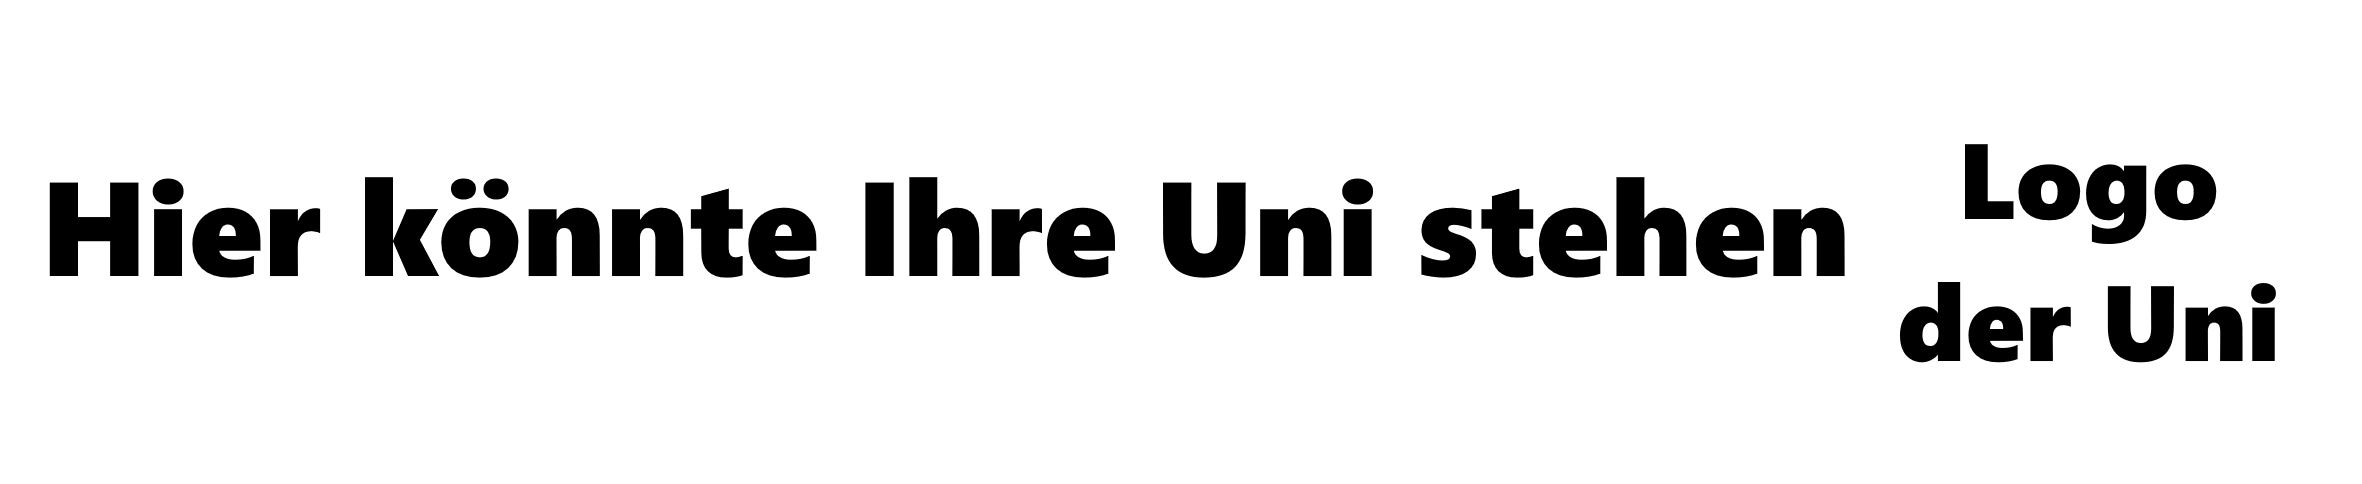
\includegraphics[height=2cm]{images/UNI_Logo.png}
\end{textblock*}
\\
\vspace*{1cm}

\begin{center}
\LARGE{\textbf{
Titel}}
\end{center}
\\

\begin{center}
\large{Abschlussarbeit zur Erlangung des akademischen Grades\\ \vspace{3mm} Bachelor/Master of Engineering (B./M. Eng.)} \\
\end{center}

\\
\begin{center}
\textbf{\Huge{Universität \\Beispielstadt\\}}
\end{center}
\\
\begin{center}
\large{\textbf{Fakultät X\\ \vspace{2mm} Studiengang Y}} 
\end{center}
\\

\begin{center}
\large{Vorgelegt von:\\ \textbf{Vorname Nachname}} \\
\large{\textbf{Matrikelnummer}}\\
\end{center}

\\

\begin{center}
\begin{tabular}{lll}
\large{Erstprüfer:} & \large Prof. Dr.-Ing. XY\\
\\
\large{Zweitprüfer:} & \large Prof. Dr.-Ing. XY\\
\\
\\
\large{Ausgegeben am:}  & \large Ausgabedatum\\
\\
\large{Abgegeben am:}  & \large Abgabedatum\\
\\
\end{tabular}
\end{center}

\end{tabular}
\end{center}
\end{singlespace}



\pagenumbering{Roman}

\phantomsection{\LARGE{\textbf{Erklärung zur Bachelor/Masterarbeit}}}
\addcontentsline{toc}{section}{Erklärung zur Bachelor/Masterarbeit}
\label{erklaerung}
\vspace*{1cm}

\vspace{1cm}

\Large{\textbf{Erklärung nach \S X Abs.\,Y Nr.\,Z APO UNI}}
\normalsize
\vspace{1cm}

Ich erkläre hiermit, dass ich die Arbeit selbstständig verfasst, noch nicht anderweitig für
Prüfungszwecke vorgelegt, keine anderen als die angegebenen Quellen oder Hilfsmittel
benutzt sowie wörtliche und sinngemäße Zitate als solche gekennzeichnet habe.

\vspace*{3.5cm}


\rule{1.0\textwidth}{0.4pt}

Ort, Datum und Unterschrift\\


\newpage

\phantomsection{\LARGE{\textbf{Kurzzusammenfassung}}}
\addcontentsline{toc}{section}{Kurzzusammenfassung}
\vspace{4mm}

\par Zusammenfassung Deutsch

\newpage
\phantomsection{\LARGE{\textbf{Abstract}}}
\addcontentsline{toc}{section}{Abstract}
\vspace{4mm}
\par Zusammenfassung Englisch

\newpage
\pagenumbering {Roman}
\pagestyle{plain}
\newpage
\setcounter{page}{4} %SEITENNUMMER EINSTELLEN

\begin{singlespace}
\vspace{10mm}
\phantomsection\addcontentsline{toc}{section}{Abkürzungsverzeichnis}
\LARGE{\textbf{Abkürzungsverzeichnis}}
\normalsize{\begin{acronym}[AMIU]
\acro{Bsp}{Beispiel}

\end{acronym}}
\end{singlespace}

\cleardoublepage

\pagenumbering{gobble}
\begin{singlespace}
\renewcommand{\contentsname}{Inhaltsverzeichnis}
\tableofcontents
\end{singlespace}
\cleardoublepage

\pagestyle{plain}

%Beginn Hauptteil

\pagenumbering {arabic}
\pagestyle{fancy}
\renewcommand{\figurename}{Abb.}

\newpage
\section{Einführung}
\label{kap:Einfuehrung}


%So ruft man Unterkapitel auf (Bestenfalls für jedes Unterkapitel eine eigene Datei anlegen)
\subsection{Zielsetzung}

\newpage
\subsection{Vorgehensweise}
\subsubsection{Noch ein Unterpunkt}

\newpage
\subsection{Was kann man mit \LaTeX{} machen?}

\par So kann man eine Abkürzung verwenden: \ac{Bsp}

\large{Erklärung zu Tabellen:}\\
\normalsize

\begin{table}[H]
\centering
\caption{Beispieltabelle.}
\label{tab:Beispieltabelle}
\begin{tabular}{ll}
\textbf{Beispiel}                      & Beispiel                      \\ \cline{2-2} 
\multicolumn{1}{l|}{Beispiel} & \multicolumn{1}{l|}{Beispiel} \\ \cline{2-2} 
\end{tabular}
\end{table}

So kann man auf \autoref{tab:Beispieltabelle} verweisen.\\
Tabelleneditor: \url{https://www.tablesgenerator.com/}\\



\Huge{\textit{So fügt man Formeln ein:}}\\
\normalsize
Formeleditor: \url{https://www.zahlen-kern.de/editor/}\\
Formeln im Fließtext: Die kinetische Energie berechnet sich wie folgt: $E_{kin} = \frac{1}{2} \cdot m \cdot v^{2}$ Die Einheit der Energie ist \textit{Joule}.

Formeln mit Numerierung:

\textbf{Übertragungsfunktion}:\\
\begin{equation}
G(s) = \frac{ y(s) }{ u(s) } = \frac{ b_{n}s^{n} + b_{n-1}s^{n-1} + \dots + b_{1}s + b_0 }{ 1s^n + a_{n-1}s^{n-1} + a_{n-2}s^{n-1} + \dots + a_{1}s+ a_0} = \frac{ Zähler }{Nenner}
\label{eq:Uebertragungsfunktion}
\end{equation}

\begin{equation}
    \begin{split}
        E_{kin} &= \frac{1}{2} \cdot m \cdot v^{2} \cr
        &= \frac{1}{2} \cdot 2\,kg \cdot (10\,\frac{m}{s})^{2} \cr
        &= 100\,J
    \end{split}
    \label{eq:Mehrzeilige_Gleichung}
\end{equation}


\newpage
\large{\textbf{Abbildungen macht man so:}}\\
\normalsize

\begin{figure}[H]
		\centering
        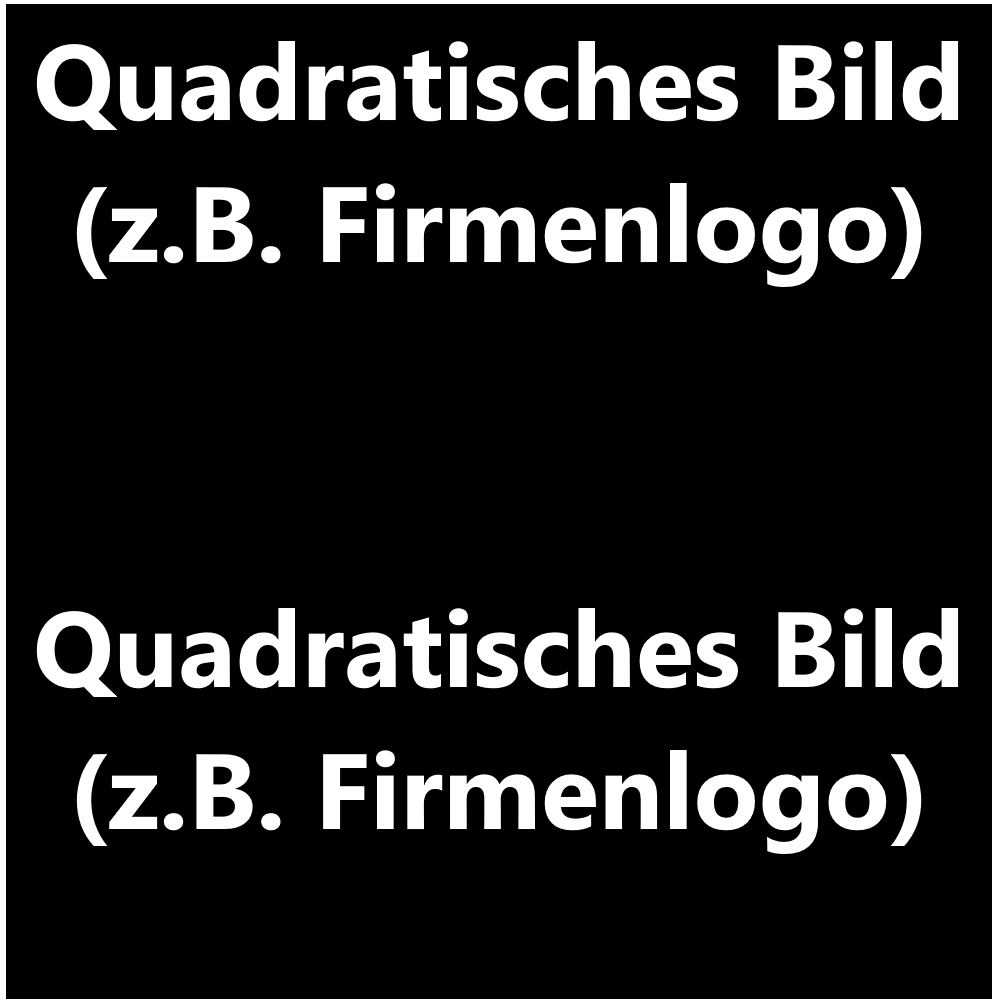
\includegraphics[width=40mm]{images/Quadrat.png}
        \caption{Hier ein wunderschönes Logo.}
        \label{abb:Panther}
\end{figure}

So kann man auf \autoref{abb:Panther} verweisen.\\

So kann man Literatur zitieren: \cite{Beispiel} \\

So verweist man auf den \nameref{label:Anhang}.


\newpage 
So springt man auf eine neue Seite und fügt ein Bild im Fließtext ein.\\

Lorem ipsum dolor sit amet, consetetur sadipscing elitr, sed diam nonumy eirmod tempor invidunt ut labore et dolore magna aliquyam erat, sed diam voluptua. At vero eos et accusam et justo duo dolores et ea rebum. Stet clita kasd gubergren, no sea takimata sanctus est Lorem ipsum dolor sit amet. Lorem ipsum dolor sit amet, consetetur sadipscing elitr, sed diam nonumy eirmod tempor invidunt ut labore et dolore magna aliquyam erat, sed diam voluptua. At vero eos et accusam et justo duo dolores et ea rebum. Stet clita kasd gubergren, no sea takimata sanctus est Lorem ipsum dolor sit amet. Lorem ipsum dolor sit amet, consetetur sadipscing elitr, sed diam nonumy eirmod tempor invidunt ut labore et dolore magna aliquyam erat, sed diam voluptua. At vero eos et accusam et justo duo dolores et ea rebum. Stet clita kasd gubergren, no sea takimata sanctus est Lorem ipsum dolor sit amet.   

\begin{wrapfigure}{r}{45mm}
  \begin{center}
        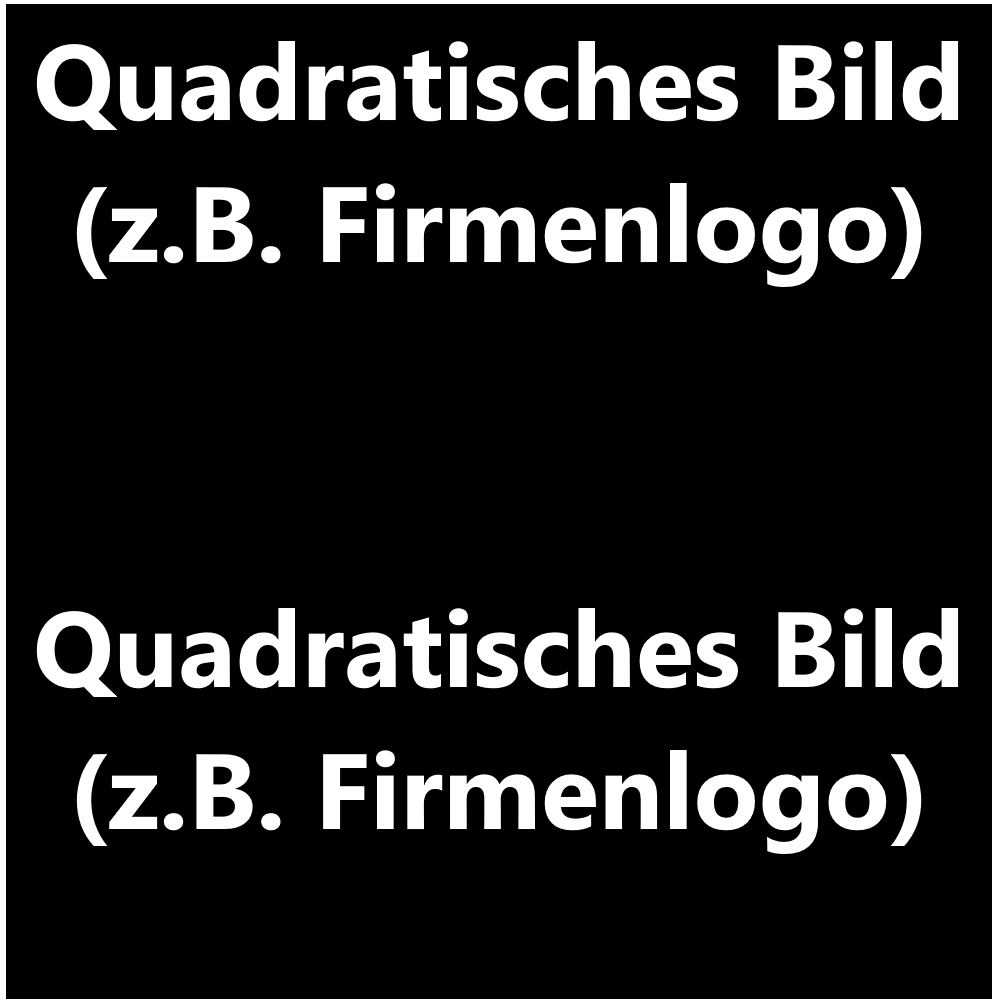
\includegraphics[width=30mm]{images/Quadrat.png}
        \caption{Hier ein wunderschönes und rechtsbündiges Logo.}
        \label{abb:Panther2}
\end{center}
\end{wrapfigure}

Duis autem vel eum iriure dolor in hendrerit in vulputate velit esse molestie consequat, vel illum dolore eu feugiat nulla facilisis at vero eros et accumsan et iusto odio dignissim qui blandit praesent luptatum zzril delenit augue duis dolore te feugait nulla facilisi. Lorem ipsum dolor sit amet, consectetuer adipiscing elit, sed diam nonummy nibh euismod tincidunt ut laoreet dolore magna aliquam erat volutpat.   

Ut wisi enim ad minim veniam, quis nostrud exerci tation ullamcorper suscipit lobortis nisl ut aliquip ex ea commodo consequat. Duis autem vel eum iriure dolor in hendrerit in vulputate velit esse molestie consequat, vel illum dolore eu feugiat nulla facilisis at vero eros et accumsan et iusto odio dignissim qui blandit praesent luptatum zzril delenit augue duis dolore te feugait nulla facilisi.   

Nam liber tempor cum soluta nobis eleifend option congue nihil imperdiet doming id quod mazim placerat facer possim assum. Lorem ipsum dolor sit amet, consectetuer adipiscing elit, sed diam nonummy nibh euismod tincidunt ut laoreet dolore magna aliquam erat volutpat. Ut wisi enim ad minim veniam, quis nostrud exerci tation ullamcorper suscipit lobortis nisl ut aliquip ex ea commodo consequat.   

Duis autem vel eum iriure dolor in hendrerit in vulputate velit esse molestie consequat, vel illum dolore eu feugiat nulla facilisis.     

\newpage
\section{Grundlagen}


%Ende Hauptteil

\newpage
\pagestyle{plain}
\pagenumbering {Roman}

\begin{singlespace}
\newpage
\setcounter{page}{6}
\phantomsection\addcontentsline{toc}{section}{Abbildungsverzeichnis}
\renewcommand{\listfigurename}{Abbildungsverzeichnis}
\listoffigures
\end{singlespace}

\begin{singlespace}
\phantomsection\addcontentsline{toc}{section}{Tabellenverzeichnis}
\renewcommand{\listtablename}{Tabellenverzeichnis}
\listoftables
\clearpage
\end{singlespace}


\newpage
\bibliographystyle{deIEEEtran}
\phantomsection\addcontentsline{toc}{section}{Literaturverzeichnis}
\renewcommand{\refname}{Literaturverzeichnis}
\bibliography{Literaturverzeichnis}
\newpage
\phantomsection{\LARGE{\textbf{\labelText{Anhang}{label:Anhang}}}}
\addcontentsline{toc}{section}{Anhang}
\label{Anhang}
\vspace*{5mm}

\large{\textbf{Beispielanhang}}
\begin{figure}[H]
    \centering
    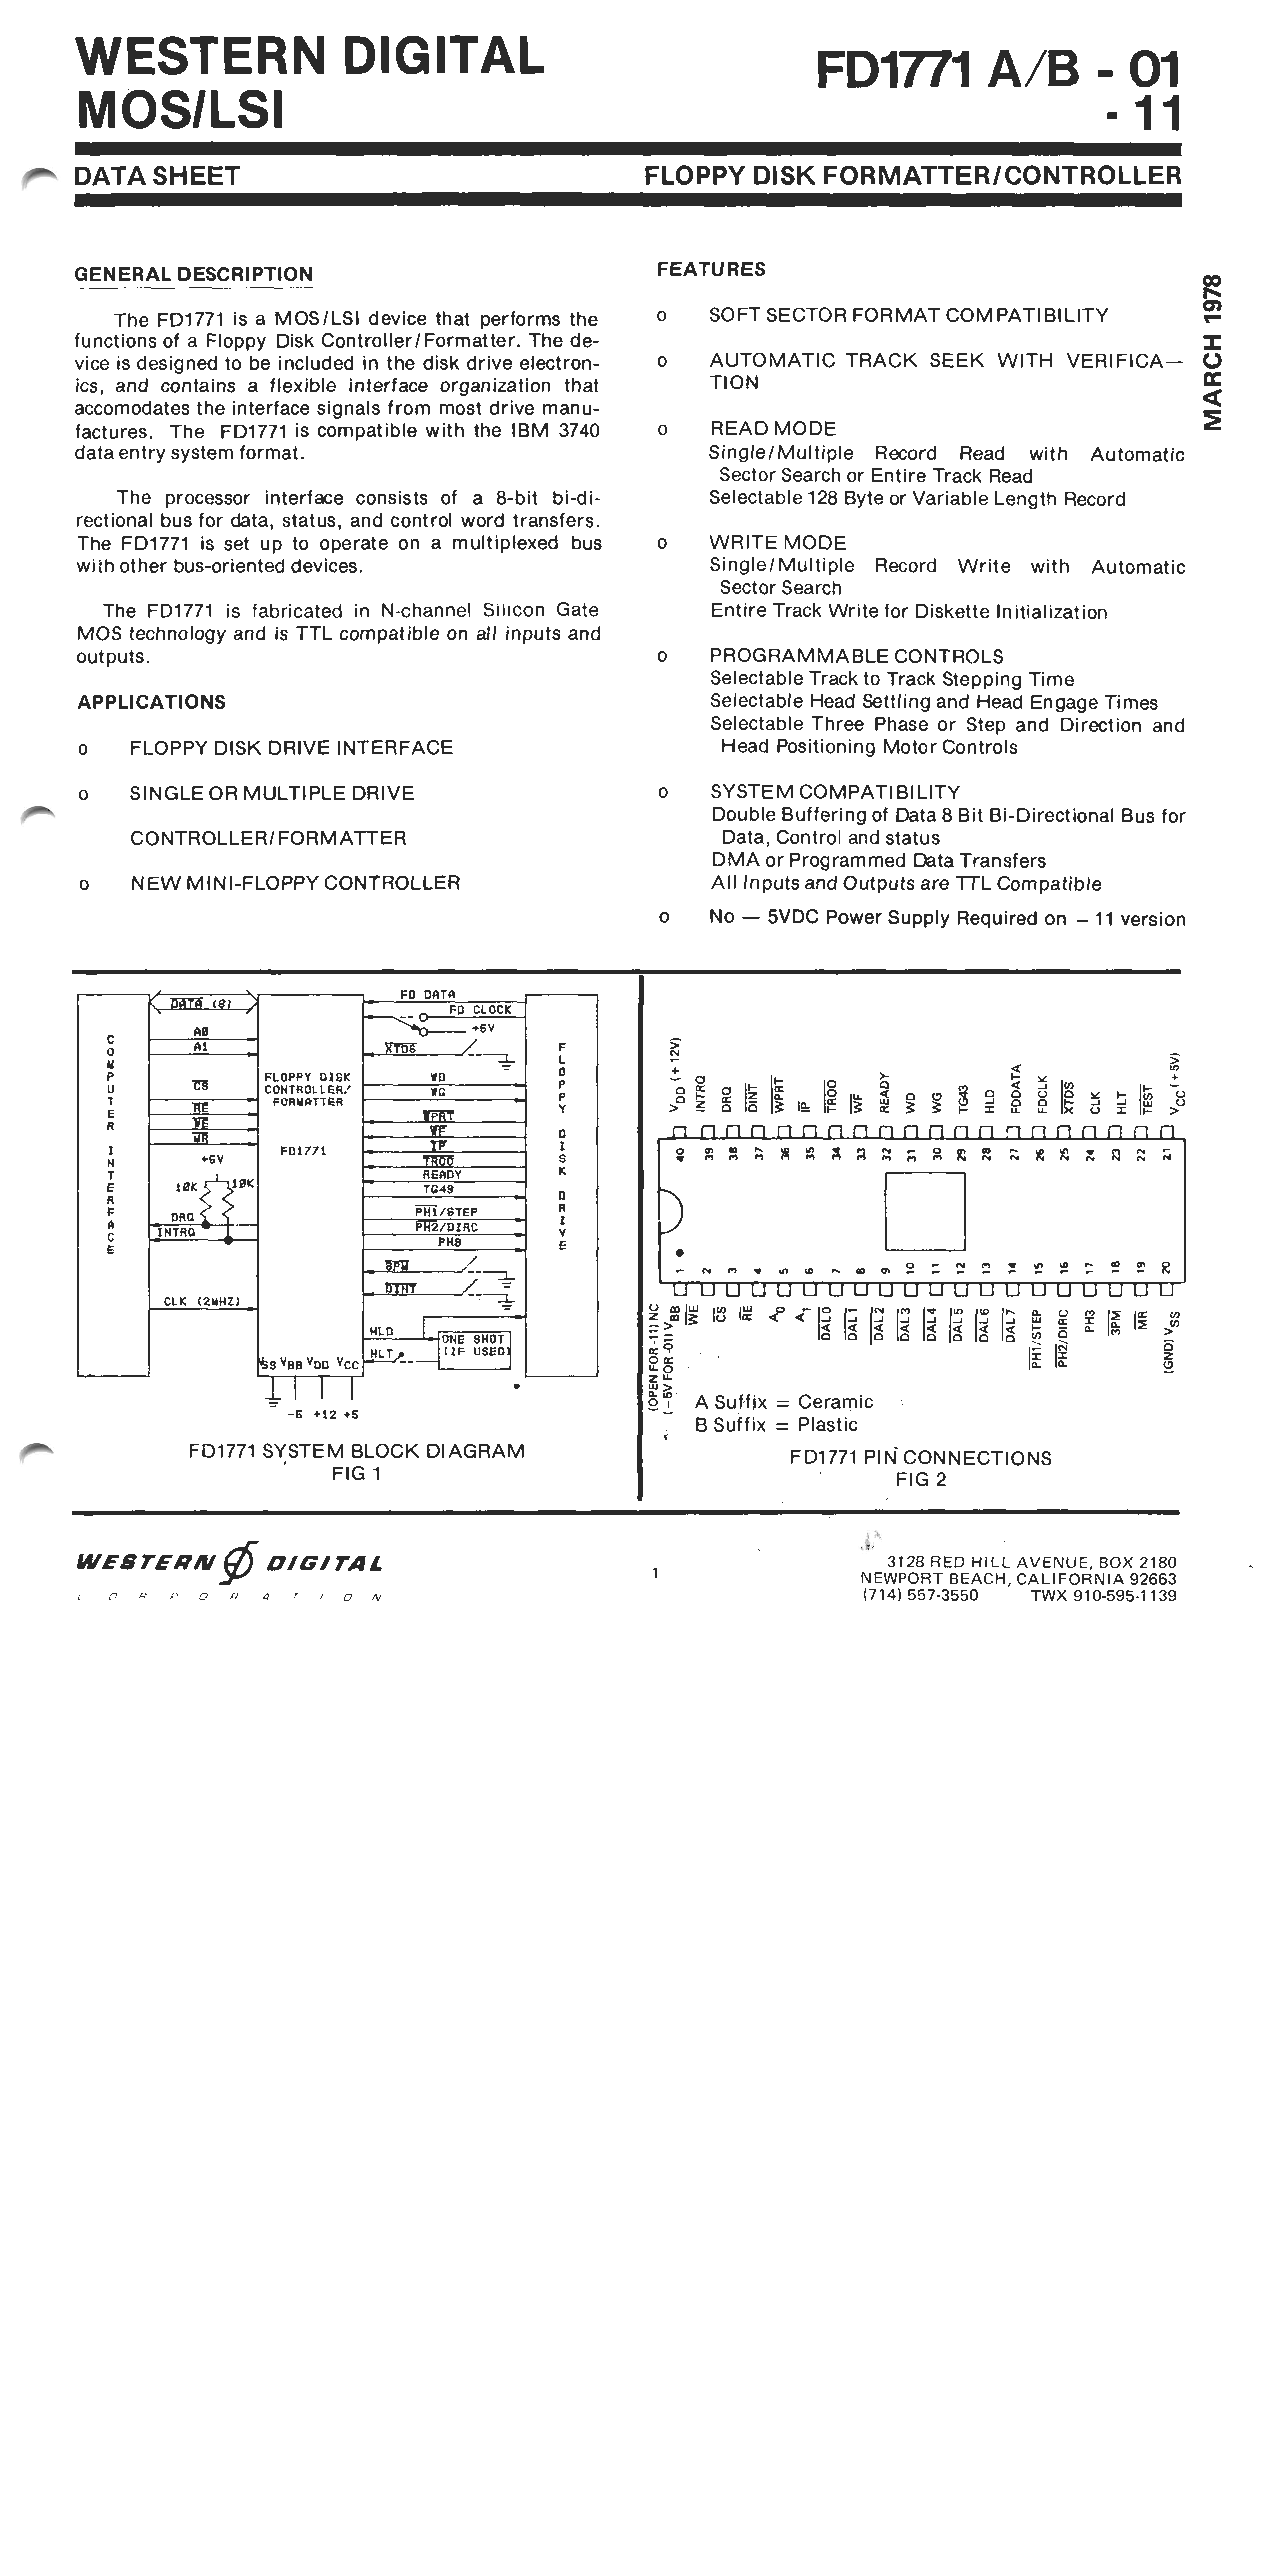
\includegraphics[width = \textwidth]{Anhang/Beispielanhang.pdf}
    \caption*{vgl. Kapitel \glqq \nameref{kap:Einfuehrung}\grqq{} - Beispielanhang.}
    \label{abb:Beispielanhang}
\end{figure} 

\end{document}